\documentclass[journal]{vgtc}               % final (journal style)
%\documentclass[review,journal]{vgtc}         % review (journal style)
%\documentclass[widereview]{vgtc}             % wide-spaced review
%\documentclass[preprint,journal]{vgtc}       % preprint (journal style)

%% Uncomment one of the lines above depending on where your paper is
%% in the conference process. ``review'' and ``widereview'' are for review
%% submission, ``preprint'' is for pre-publication, and the final version
%% doesn't use a specific qualifier.

%% Please use one of the ``review'' options in combination with the
%% assigned online id (see below) ONLY if your paper uses a double blind
%% review process. Some conferences, like IEEE Vis and InfoVis, have NOT
%% in the past.

%% Please note that the use of figures other than the optional teaser is not permitted on the first page
%% of the journal version.  Figures should begin on the second page and be
%% in CMYK or Grey scale format, otherwise, colour shifting may occur
%% during the printing process.  Papers submitted with figures other than the optional teaser on the
%% first page will be refused. Also, the teaser figure should only have the
%% width of the abstract as the template enforces it.

\pagestyle{plain}

%% These few lines make a distinction between latex and pdflatex calls and they
%% bring in essential packages for graphics and font handling.
%% Note that due to the \DeclareGraphicsExtensions{} call it is no longer necessary
%% to provide the the path and extension of a graphics file:
%% 
\includegraphics{diamondrule} is completely sufficient.
%%
\ifpdf%                                % if we use pdflatex
  \pdfoutput=1\relax                   % create PDFs from pdfLaTeX
  \pdfcompresslevel=9                  % PDF Compression
  \pdfoptionpdfminorversion=7          % create PDF 1.7
  \ExecuteOptions{pdftex}
  \usepackage{graphicx}                % allow us to embed graphics files
  \DeclareGraphicsExtensions{.pdf,.png,.jpg,.jpeg} % for pdflatex we expect .pdf, .png, or .jpg files
\else%                                 % else we use pure latex
  \ExecuteOptions{dvips}
  \usepackage{graphicx}                % allow us to embed graphics files
  \DeclareGraphicsExtensions{.eps}     % for pure latex we expect eps files
\fi%

%% it is recomended to use ``\autoref{sec:bla}'' instead of ``Fig.~\ref{sec:bla}''
\graphicspath{{figures/}{pictures/}{images/}{./}} % where to search for the images

\usepackage{microtype}                 % use micro-typography (slightly more compact, better to read)
\PassOptionsToPackage{warn}{textcomp}  % to address font issues with \textrightarrow
\usepackage{textcomp}                  % use better special symbols
\usepackage{mathptmx}                  % use matching math font
\usepackage{times}                     % we use Times as the main font
\renewcommand*\ttdefault{txtt}         % a nicer typewriter font
\usepackage{cite}                      % needed to automatically sort the references
\usepackage{tabu}                      % only used for the table example
\usepackage{booktabs}                  % only used for the table example
%% We encourage the use of mathptmx for consistent usage of times font
%% throughout the proceedings. However, if you encounter conflicts
%% with other math-related packages, you may want to disable it.

%% In preprint mode you may define your own headline.
%\preprinttext{To appear in IEEE Transactions on Visualization and Computer Graphics.}

%% If you are submitting a paper to a conference for review with a double
%% blind reviewing process, please replace the value ``0'' below with your
%% OnlineID. Otherwise, you may safely leave it at ``0''.
\onlineid{0}

%% declare the category of your paper, only shown in review mode
\vgtccategory{Research}
%% please declare the paper type of your paper to help reviewers, only shown in review mode
%% choices:
%% * algorithm/technique
%% * application/design study
%% * evaluation
%% * system
%% * theory/model
\vgtcpapertype{please specify}

%% Paper title.
\title{INM460 Computer Vision - Coursework Report}

%% This is how authors are specified in the journal style

%% indicate IEEE Member or Student Member in form indicated below
\author{Daniel Sikar - MSc Data Science PT2}
\authorfooter{
%% insert punctuation at end of each item
\item
 Daniel Sikar, City University of London, daniel.sikar@city.ac.uk
}


%%%%%%%%%%%%%%%%%%%%%%%%%%%%%%%%%%%%%%%%%%%%%%%%%%%%%%%%%%%%%%%%
%%%%%%%%%%%%%%%%%%%%%%%%%% ABSTRACT %%%%%%%%%%%%%%%%%%%%%%%%%%%%
%%%%%%%%%%%%%%%%%%%%%%%%%%%%%%%%%%%%%%%%%%%%%%%%%%%%%%%%%%%%%%%%

%% \input{INM460-final-report-0.5-abstract.tex}

%%%%%%%%%%%%%%%%%%%%%%%%%%%%%%%%%%%%%%%%%%%%%%%%%%%%%%%%%%%%%%%%
%%%%%%%%%%%%%%%%%%%%%%%%%% KEYWORDS %%%%%%%%%%%%%%%%%%%%%%%%%%%%
%%%%%%%%%%%%%%%%%%%%%%%%%%%%%%%%%%%%%%%%%%%%%%%%%%%%%%%%%%%%%%%%

%% Keywords that describe your work. Will show as 'Index Terms' in journal
%% please capitalize first letter and insert punctuation after last keyword
\keywords{Person Identification, CNN, HOG, SURF, SVM}

%% Uncomment below to include a teaser figure.
\teaser{
  \centering
  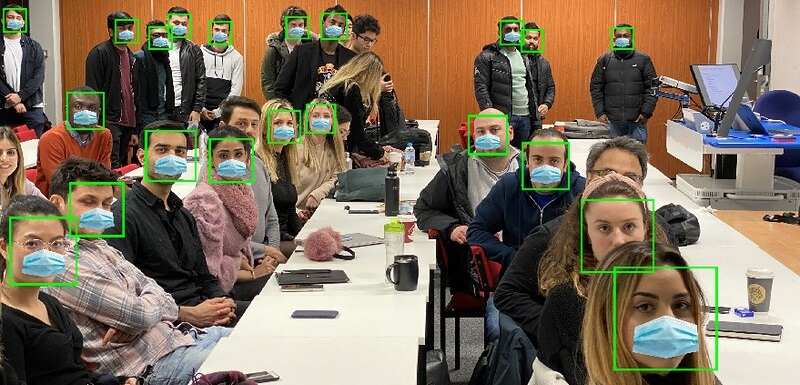
\includegraphics[width=\linewidth]{inm460-classroom.jpg}
  \caption{Creative Mode processing of INM460 coursework classroom image}
	\label{fig:teaser}
}

%% Uncomment below to disable the manuscript note
\renewcommand{\manuscriptnotetxt}{}

%% Copyright space is enabled by default as required by guidelines.
%% It is disabled by the 'review' option or via the following command:
% \nocopyrightspace

%\vgtcinsertpkg

%%%%%%%%%%%%%%%%%%%%%%%%%%%%%%%%%%%%%%%%%%%%%%%%%%%%%%%%%%%%%%%%
%%%%%%%%%%%%%%%%%%%%%% START OF THE PAPER %%%%%%%%%%%%%%%%%%%%%%
%%%%%%%%%%%%%%%%%%%%%%%%%%%%%%%%%%%%%%%%%%%%%%%%%%%%%%%%%%%%%%%%%

\begin{document}

%% The ``\maketitle'' command must be the first command after the
%% ``\begin{document}'' command. It prepares and prints the title block.

%% the only exception to this rule is the \firstsection command

%\firstsection{ProjectOverview}

\maketitle

%%%%%%%%%%%%%%%%%%%%%%%%%%%%%%%%%%%%%%%%%%%%%%%%%%%%%%%%%%%%%%%%
%%%%%%%%%%%%%%%%%%%%%% INTRODUCTION %%%%%%%%%%%%%%%%%%%%%%%%%%%%
%%%%%%%%%%%%%%%%%%%%%%%%%%%%%%%%%%%%%%%%%%%%%%%%%%%%%%%%%%%%%%%%

%% Project Overview goes here
\section{Overview}

This INM460 Computer Vision coursework project consists of creating facial classifiers from supplied image stills and videos of two types: individual and group, labelled and unlabelled respectively as shown in Fig. \ref {fig:data_example}.
\begin{figure}[h]
 \centering 
 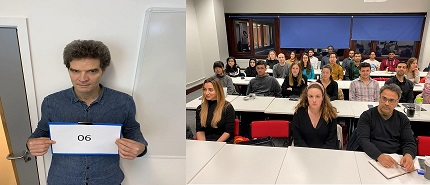
\includegraphics[width=\columnwidth]{images/example-data-50pc.jpg}
 \caption{Example of individual (labelled) and group (unlabelled) images}
 \label{fig:data_example}
\end{figure}

Each individual image contains a sign with a two-digit unique identifier, from which labelled data is obtained to train and test classifier models. 
\subsection{Pre-processing Steps}
For our coursework, the chosen programming language was MATLAB \cite{MATLAB:2018}, version 2018a. All pre-processing steps were sequentially run in script \textbf{ImagePreProcessing.m}, using MATALB user-defined functions:
\begin{enumerate}
\item fnSaveVideoStills
\item fnLabelIndividualImages
\item fnBlurImages
\item fnRotateImages
\item fnCropFaces
\end{enumerate}
In step 1. all videos were saved as stills, with the exception of beginning and ending frames of each video, which were normally black or excessively blurred. In step 2. all images containing unique identifiers which could be recognised through optical character recognition (OCR) with our function \textbf{fnGetStudentID} were moved to a labelled folder, otherwise set aside for manual labelling. Once all images had been identified and moved to labelled folders, totalling 48 labels, we obtained an average of 402 images per label. In steps 3. and 4. the entire data then was augmented by randomly selecting 50\% of each label and applying a random amount of blur to each image, then a further 70\% was randomly selected from each label (including recently added blurred images) and randomly rotated from -10 to 10 degrees.  

The augmented data after step 4. had an average of 1026 images per label. In Step 5. faces were cropped, using MATLAB's vision.CascadeObjectDetector which implements the Viola-Jones algorithm  \cite{990517}, and moved to another set of labelled folders. An average of 985 faces were obtained from each label, which represents approximately 96\% of the augmented data.  
Each label was then manually checked and any images not correctly cropped were removed, resulting in an average of 815 images per label, doubling the size of face image data with respect to stills obtained in step 2. Table \ref {table:preproc} shows label quantities after each processing step, including totals and averages per label.
\begin{table}[h]
\centering
\begin{tabular}{|l|l|l|l|l|l|}
\hline
\multicolumn{6}{|l|}{Pre-processing figures} \\ \hline
Step  &  2 & 3 & 4 & 5 & Final\\ \hline
Total images & 19323 & 28984 & 49273 & 47302 & 39135 \\ \hline
Label avg. & 402 & 604 & 1026 & 985 & 815  \\ \hline
\end{tabular}
\caption{Label quantities after each pre-processing step}
\label{table:preproc}
\end{table}
Fig. \ref {fig:cropped_example} shows examples of three correct face crops, without and with augmentation, and one shoe incorrectly identified as a face.

\begin{figure}[h]
 \centering 
 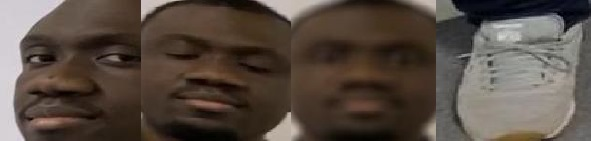
\includegraphics[width=\columnwidth]{images/crop-examples.jpg}
 \caption{Cropped face images including augmented rotated, augmented blurred and misidentified}
 \label{fig:cropped_example}
\end{figure}

\subsection{Determining optimal cropped-face size}

To determine what image size to use for training our models, we examined individual and group images. Files resulting from pre-processing step 5. were square, with varying side dimensions. We used function \textbf{fnStatsCropSizes.m} to calculate the minimum, maximum, median and mode averages of the side of the cropped-face square image (Table \ref{table:face_crop_stats}). 

\begin{table}[h]
\centering
\begin{tabular}{|l|l|l|l|}
\hline
\multicolumn{4}{|l|}{Individual face image side size statistics} \\ \hline
Minimum  &  Maximum & Median & Mode \\ \hline
100 & 252 & 171 & 152 \\ \hline
\end{tabular}
\caption{Rounded average size in pixels for pre-processed images over all labels}
\label{table:face_crop_stats}
\end{table}

We then looked at faces found in group images, both still images, and still images obtained from videos. The latter proved mostly unusable, as the amount of blur did not allow for more than 2 or 3 face images being identified in each frame, so group videos were discarded. We used function \textbf{fnStatsGroupCropSizes.m} to identify face sizes in still group images and obtained cropped face statistics (Table \ref{table:group_crop_stats}).

\begin{table}[h]
\centering
\begin{tabular}{|l|l|l|l|}
\hline
\multicolumn{4}{|l|}{Group face image side size statistics} \\ \hline
Minimum  &  Maximum & Median & Mode \\ \hline
100 & 322 & 128 & 107 \\ \hline
\end{tabular}
\caption{Rounded average size in pixels for pre-processed images over all group images}
\label{table:group_crop_stats}
\end{table}

Since the median side size from faces cropped from group images was 128 and the mode was 107, and group images were the unlabelled data we are looking at classifying, intuitively it seemed to make sense to resize all labelled images closer to the minimum end of the size range, which would require the least amount of resizing to train and test our models, particularly aiming at avoiding to increase the size of cropped faces from group images, introducing some amount of blur. As an example, Figure \ref{fig:decrease_increase_example} shows a sequence where an image of size 217x217 pixels is decreased to size 115x115, with no loss of sharpness, then resized again to 227x227, with some loss of sharpness.

\begin{figure}[ht]
 \centering 
 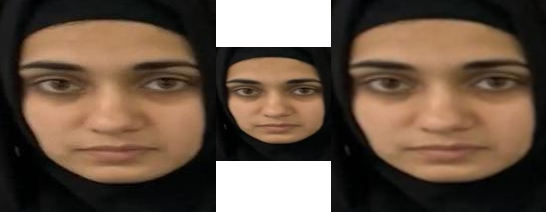
\includegraphics[width=\columnwidth]{images/decrease-increase.png}
 \caption{Sequence showing the effect of decreasing and increasing cropped-face images sizes, from left to right, image is decreased with no apparent loss in sharpness, then increased with some loss in sharpness}
 \label{fig:decrease_increase_example}
\end{figure}

We used function \textbf{fnGetSampleImages.m} to generate sample data for initial models, and based on the results, expanded to full data. We worked with random sets of 50, 100 and 200 images from 8 labels, in three different sizes 227x227, 128x128 and 70x70 pixels, both RGB and grayscale, and then created a few models to test our hypothesis.  

Since a visual inspection showed numerous repetitions in each label, a sample size of 200 images per label was considered sufficient to generate the classifiers.





%%%%%%%%%%%%%%%%%%%%%%%%%%%%%%%%%%%%%%%%
%% DESCRIPTION OF IMPLEMENTED METHODS %%
%%%%%%%%%%%%%%%%%%%%%%%%%%%%%%%%%%%%%%%%

\section{Description of implemented methods}
\label{DOIM-marker} 
Three face recognition feature-classifier types were implemented: Convolutional Neural Network (CNN), Histogram of Oriented Gradients and Support Vector Machine (HOG-SVM) and Speeded-up Robust Features and Support Vector Machine (SURF-SVM), mostly based on code covered in labs, with some adaptations for HOG-SVM and SURF-SVM, as well as CNN for grayscale images. A gridsearch was run for each method, aiming to find optimal image sizes, colour schemes and some parameter tuning for HOG-SVM and SURF-SVM. Script \textbf{TrainNetworks.m} was used for the grid searches and to generate classifiers, confusion matrices and statistics, by looping through all parameters being tested for each classifier. Best performing classifiers for labelled individual image dataset, tested on 980 images, are displayed in Table \ref{table:acc_table}.
\begin{table}[h]
\centering
\begin{tabular}{|l|l|l|}
\hline
\multicolumn{3}{|l|}{Accuracy of face recognition models} \\ \hline
Feature-Classifier  &  Name & Accuracy \\ \hline
CNN & dan\_net\_70\_rgb & 0.9990 \\ \hline
HOG-SVM & HOGSVMMdl\_70x70 & 0.9990 \\ \hline
SURF-SVM & SURFSVMMdl\_70px\_50pt & 0.8656 \\ \hline
\end{tabular}
\caption{Accuracy table for labelled individual images}
\label{table:acc_table}
\end{table}
We then tested each classifier on 5 group images. We used function \textbf{RecogniseFace} which identified a total of 101 faces, then computed the accuracies manually. Results are shown in Table \ref{table:acc_table_group}.
\begin{table}[h]
\centering
\begin{tabular}{|l|l|l|}
\hline
\multicolumn{3}{|l|}{Accuracy of face recognition models} \\ \hline
Feature-Classifier  &  Name & Accuracy \\ \hline
CNN & dan\_net\_70\_rgb & 0.1386 \\ \hline
HOG-SVM & HOGSVMMdl\_70x70 & 0.1287 \\ \hline
SURF-SVM & SURFSVMMdl\_70px\_50pt & 0.1188 \\ \hline
\end{tabular}
\caption{Accuracy table for group images}
\label{table:acc_table_group}
\end{table}



%% CNN

\subsection{CNN}
\label{CNN-label}

Our Convolutional Neural Network image classifier was our best model by a narrow margin. We do not include a block diagram of the key algorithmic components as the image processing was quite simple and limited to augmentation consisting of blurring and rotation.  

Our network was based on lab code \cite{INM460-lab-wk8}. Some alternative network architectures were tried, with added layers, different learning rates and epochs. We could not improve on the network given in class and in the end used it without modification, that is, two stacks of convolutional, batch normalization, rectified linear unit and max pooling layers, followed by the same stack excluding max pooling layer, followed by a fully connected, softmax and classification layer. For grayscale images, we changed the dimensions of the image input layer, to account for the single colour channel.

We varied training epochs from 2 to 32 and found that 4 was an adequate number (Figure \ref{fig:cnn_training_progress} - dark continuous curve: training accuracy smoothed, light continuous curve: training accuracy, dashed lines: validation accuracy), as the network had usually converged by then to a stable accuracy value that was unlikely to change with the addition of more epochs.

\begin{figure}[h]
 \centering 
 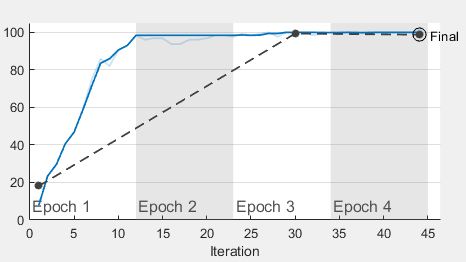
\includegraphics[width=\columnwidth]{images/cnn-training-progress.png}
 \caption{CNN training progress showing conversion after three epochs, for 200 samples per label, 128x128 pixel RGB images}
 \label{fig:cnn_training_progress}
\end{figure}

We used function \textbf{fnTrainCNN} to train our networks. This returned the trained network and accuracy as output parameters, used to build Table \ref{table:cnn_stats} in section \ref{Appendix}. The outputs showed that our networks worked better with smaller images, consistently generating higher accuracies for grayscale image sizes of 70x70 pixels. Overall, networks trained using grayscale images performed slightly better than the RGB counterparts on individual images, which suggests variability such as introduced by differing light conditions might have been attenuated in grayscale images. 

We tried using grayscale images as a single channel input to our convolutional neural network as they trained faster than 3 channel RGB images. We tested our grayscale image network on one group image (class2.jpg), using our \textbf{RecogniseFace} function. One in twenty images was classified correctly. Compared to 4 in 20 using our best RGB model. The reason for the lower performance of grayscale images on group images may be related to further processing being required in group images, as performance on individual images was better for grayscale than RGB images. We discuss this in section \ref{Discussion-marker}.

Based on ad hoc testing and grid search results, 70x70 pixel RGB images were chosen to train the coursework CNN models. Figure \ref{fig:cnn_correct_incorrect} shows a detail of image generated by our \textbf{RecogniseFace} function with one correct and one incorrect classification
\begin{figure}[ht]
 \centering 
 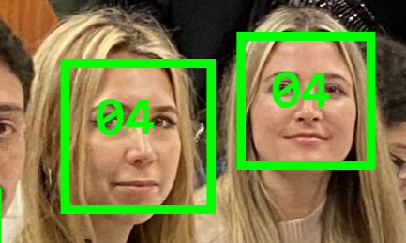
\includegraphics[width=\columnwidth]{images/correct-incorrect.png}
 \caption{Correct (left) and incorrect (right) classification labels from CNN trained with 70x70 pixel RGB images}
 \label{fig:cnn_correct_incorrect}
\end{figure}



%% HOG-SVM

\subsection{HOG-SVM}  
For our HOG-SVM feature type / classifier combination we used locally normalized histogram of oriented gradients (HOG) descriptors \cite{citeulike:335784} as the feature type and a multiclass model for support vector machine as the classifier. The method takes an input image which is normalized for gamma and colour for better invariance to factors such as illumination and shadowing, then a grid is placed on the image and for every cell a histogram of oriented gradient features is extracted, the concept being local object appearance and shape are characterized by a distribution of intensity gradients or edge positions. Each cell holds a 1-D histogram of gradients and edge orientations over the pixel of the cell, noting that the referenced work applied to human detection in general. 

We defined function \textbf{fnCreateHOGSVMClassifier} to create a multiclass model for support vector machine using matlab function \textbf{fitcecoc}, and script \textbf{TrainNetworks.m} to test different classifiers, using code supplied in lab 6 \cite{INM460-lab-wk6} with some modifications. Data was split at a ratio of 90\%/10\% for training and testing. Training data was then run through the feature extraction function  \textbf{extractHOGFeatures}, which generated our encoded shape information. Since we had to somehow turn the features into a vector to be used by our Support Vector Machine classifier, we chose to use grayscale images as the intuition was this approach would constrain the task and make it more manageable - see section \ref{Discussion-marker}. We tested different cell sizes; [50 50], [25 25] and [10 10], finding that smaller cell sizes generated a larger number of HOG features, as well as higher accuracies. The data generated from our grid search is shown in Table \ref{table:hog_stats}, section \ref{Appendix}. Given the feature length was not necessarily the same for each image and smaller cell sizes generated more features, we defined a value of 2500 features, which in most cases exceeded the number of features extracted for each image. We then used this value to adjust the size of the vector that would be used to train our SVM. If the feature vector returned by \textbf{extractHOGFeatures} was greater, we shortened the vector, and if it was less, we padded the feature vector with zeros, to ensure the final feature vector was always equal to our defined feature size.

The same process, as implemented in function \textbf{fnHOGSMVPredict}, was used when classifying unseen group images. HOG features were extracted, vector size adjusted before being passed to the SMV classifier.

Our best HOG-SVM model accuracy was 0.9990 (Table \ref{table:acc_table}). Since we had a total of 48 labels, the resulting confusion matrix was not readable, so we created a subset with 8 labels with the same 200 images for each label, generating the confusion matrix shown in Figure \ref{fig:hog_conf_mat} with approximately the same accuracy. 

\begin{figure}[h]
 \centering 
 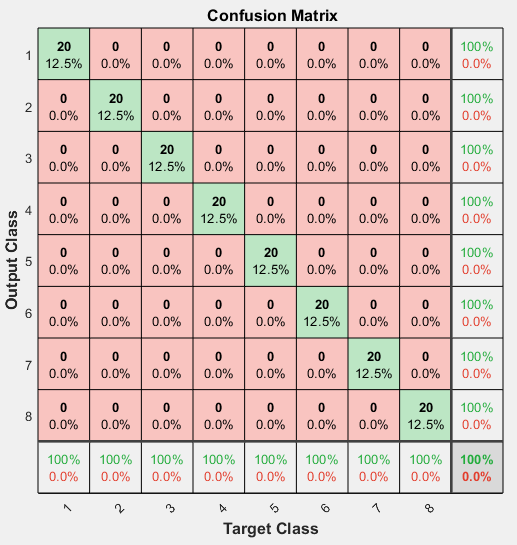
\includegraphics[width=\columnwidth]{images/HOG-SVM-Conf-Mat-200-gray-0.9.png}
 \caption{HOG SVM Confusion Matrix, 8 labels, 200 images each, 90\%/10\% train/test split}
 \label{fig:hog_conf_mat}
\end{figure}  
The widely different accuracy obtained from testing individual labelled images and testing group images (Tables \ref{table:acc_table} and \ref{table:acc_table_group}) suggests the model is overfitting. We discuss this in section \ref{Discussion-marker}.




%% SURF-SVM

\subsection{SURF-SVM}  
SURF uses the concept of interest points (as covered in lecture 5) as a means to build a set of features that will later help establish a correspondence between two images. SURF uses windows (somewhat analogous to HOG cells), which are divided into subregions, and further subdivided into grids. By using Haar wavelets pixel intensity sums, a 4-number descriptor is obtained to define a subregion \cite{Bay2008346}.  

We used MATLAB functions \textbf{detectSURFFeatures}  to obtain SURF features and \textbf{extractFeatures} to obtain descriptors. Once again we observed that different images generated different feature numbers, so applied the same principle used to generate our HOG-SVM classifier. We used script \textbf{TrainNetworks.m} and function \textbf{fnCreateSURFSVMClassifier} to try out different parameters; results shown in Table \ref{table:surf_stats}, section \ref{Appendix}. We opted to use 50 SURF features with 200 70x70 grayscale images, as RGB images could not be used. This was not our best performing model but for the sake of having a single data for the HOG-SVM and SURF-SVM classifiers we sacrificed SURF-SVM accuracy. See section \ref{Discussion-marker} for discussion.   

To generate the matrix to fit our multiclass models for our support vector machine, we used the same approach as with our HOG-SVM, except the final vector adjustment had a slightly different implementation, to account for the 64 dimensions used in SURF.

To run our SURF-SVM classifier we used function \textbf{fnSURFSMVPredict}, again using the same principle as with the HOG-SVM classifier, where the same SURF feature number is used to make predictions, as was used to fit the classifier.  

The final SURF-SVM classifier accuracy obtained from fitting a model with 50 SURF features, 48 labels and 200 70x70 pixel grayscale images was 0.90625 (Table \ref{table:surf_stats}, section \ref{Appendix}). The confusion matrix for our best model was unreadable due to the amount of rows and columns, so we generated a second confusion matrix with 8 labels only (Figure \ref{fig:surf_conf_mat}). The accuracy obtained for the 8-label model was 96.3\%. This is assumed to be an artifact, due to individual labels presenting different classification accuracies.

\begin{figure}[h]
 \centering 
 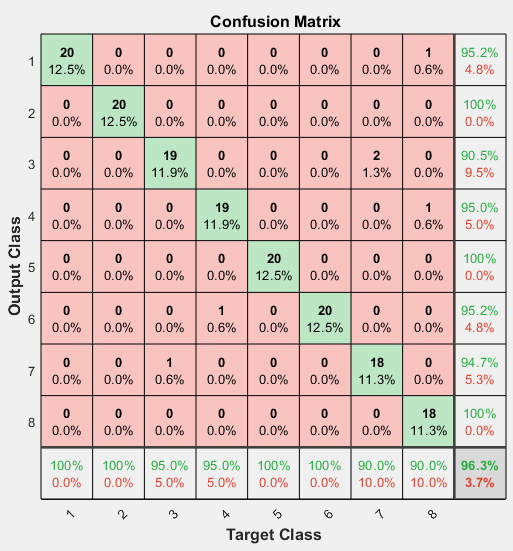
\includegraphics[width=\columnwidth]{images/SURF-SVM-Conf-Mat-200-gray-0.9.png}
 \caption{SURF SVM Confusion Matrix, 8 labels, 200 images each, 90\%/10\% train/test split}
 \label{fig:surf_conf_mat}
\end{figure} 


%% Creative Mode

\subsection{Creative Mode}
For the creative mode task we chose to place a face mask on every face found in an image. This was implemented in function \textbf{fnPandemicMode}. 
 
We used the \textbf{roipoly} method to define a polygonal region of interest in the original face mask image (facemask-cropped.jpg). we then scaled the face mask image and the polygonal region of interest with respect to cropped face image size. We then created "positive" and "negative" segmentation mask matrices, to add or remove the face mask image or region as required. The dot product between the cropped face image and the negative mask matrix removed the face mask region, all black colour values in that region being equal to zero. This resulting matrix was then added to the positive mask, containing the face mask image surrounded by a blacked out region.  

To define where the mask would be placed, our initial approach was to use a mouth locating feature from MATLAB object \textbf{vision.CascadeObjectDetector}. We did not find this approach robust, as returned mouth locations varied between nose and chin. In the end we found it simpler to display the mask at a fixed ratio from the bottom edge and mid-point between side edges of cropped face.

On the top row of Figure \ref{fig:pandemic_mode}, the middle image represents the negative segmentation mask. A dot product with the cropped face on left-hand size image creates a black void in the face mask area on right-hand side image. On the bottom row, the middle image represents the positive segmentation mask, which is added to "voided" left-hand side image, resulting in void being filled by face mask on right-hand side image. These were the concepts used for prototyping, in practice we removed a section from cropped face, performed the matrix operations and inserted the resulting section back into the original image.

\begin{figure}[h]
 \centering 
 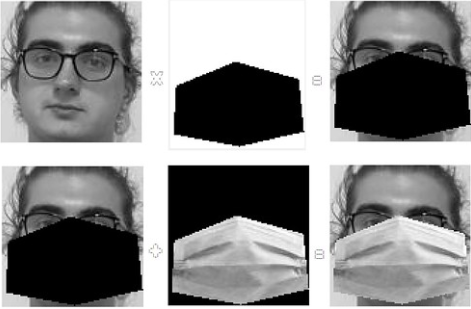
\includegraphics[width=\columnwidth]{images/PandemicMode.png}
 \caption{Creative Mode superimposing facemask on face image}
 \label{fig:pandemic_mode}
\end{figure}

%% Discussion

\section{Discussion}
\label{Discussion-marker}
This coursework project had a variety of tasks which required a good level of organisation, from data pre-processing onwards. Therefore it also turned out an exercise in time management and resource allocation.  

Organising the image training sets, which seemed to be a minor task, turned out to be major, and provided an appreciation for what projects like ImageNet \cite{imagenet_cvpr09} must have been like.  

The original SURF paper \cite{Bay2008346} does account for RGB images being used, though the MATLAB implementation of detectSURFFeatures only accepts grayscale images. Future work with the HOG-SVM and SURF-SVM classifiers could include using RGB images to generate HOG and SURF features, by encoding each channel separately and to a fixed length channel vector as per single channel grayscale images, then stacking channels sequentially, such that the vector would always have the channel features in the same vector indices. 

One of SURF's strengths is finding descriptors invariant to orientation change, which we could have tested by not rotating images in our training set, then using rotated images in our test set. Under such conditions, we would expect that SURF-SVM might gain on the CNN and HOG-SVM classifiers.

We did not use the best possible SURF-SVM model for the sake of using a common set of images for both HOG-SVM and SURF-SVM.

The different accuracy obtained by testing on unseen individual images and unseen group images suggests overfitting may have occurred. We tested different splits for SURF-SVM models (which presented the lowest accuracy) of 80/20 and 70/30 without substantial change in accuracy observed for testing data. We assumed that, if all three classifiers - CNN HOG-SVM and SURF-SVM - were indeed overfitting, one cause may be there is a limited amount of variability that can be introduced by augmentation, and ending up with 200 sample images for every label may be the cause. Further splits would be required to determine if this was indeed the case. The expectation being, if an unorthodox split of 30/70 was tried and the accuracies for individual image classification were still high, this would confirm the hypothesis.  

Also, in terms of training/testing splits, K-fold cross-validation might help with establishing if the data was somehow impoverished by our augmentation.

Another cause of the model accuracy discrepancy between test individual and group images, may be due to group images not being representative enough. This may be a shortcoming of our processing pipeline, that might have benefited from trying to approximate individual and group image characteristics such as contrast.

We were not able to implement a confidence measure for HOG-SVM and SURF-SVM classifiers, so all labels generated by both classifiers have an ID, unlike our CNN classifier which shows an ID relative to a confidence measure.

Adding a confidence measure to HOG-SVM and SURF-SVM classifiers could be generated by using a measure of distance to the classification boundary. Further refinements, such as the use of multiple models and "voting" schemes could be one option, whereby the output labels from each model would be grouped and summed and the highest number chosen as the output label.

Producing the HOG-SVM and SURF-SVM classifiers was the highlight of this project and one of the highlights of my time at City so far, as it is the culmination of practical and theoretical knowledge obtained since joining the programme. The CNN classifier was expected to outperform both HOG-SVM and SURF-SVM. The fact that HOG-SVM matched the CNN classifier in performance and the SURF-SVM did quite well was a surprise in the true spirit of research, where the outcome is never certain.

%%%%%%%%%%%%%%%%%%%%%%%%%%%%%%%%%%%%%%%%%%%%%%%%%%%%%%%%%%%%%%%%
%%%%%%%%%%%%%%%%% Findings and Reflections %%%%%%%%%%%%%%%%%%%%%
%%%%%%%%%%%%%%%%%%%%%%%%%%%%%%%%%%%%%%%%%%%%%%%%%%%%%%%%%%%%%%%%

%\section{Discussion}

We processed our data by transforming hexadecimal encoded byte values into numerical valued between 0 and 255 (unsigned bytes) as well as all the bit flags present in our flame detector units under test. We isolated two files (Test45.log, Test48.log) and a further representative section within these files, representing signal (fire) and noise (interference). Both sets of data plotted as Flame A detector, Flame B detector and Guard as discussed in Jupyter Notebook.

\subsection{Signal data}

We plotted our signal data finding that the fire event generated values for Flame Detector A and Flame detector B that closely overlapped.

\begin{figure}[tb]
 \centering % avoid the use of \begin{center}...\end{center} and use \centering instead (more compact)
 \includegraphics[width=\columnwidth]{pictures/01-real-fire-data.png}
 \caption{Closely overlapping Flame A and Flame B fire data}
 \label{fig:sample}
\end{figure}

\subsection{Noise data}

We plotted the same section of our noise data and found that Flame A and Flame B did not overlapped, in fact in parts they were going in opposite directions (antiphase), finding that this could become an engineered feature.

\begin{figure}[tb]
 \centering % avoid the use of \begin{center}...\end{center} and use \centering instead (more compact)
 \includegraphics[width=\columnwidth]{pictures/02-interference-data.png}
 \caption{Interference plot, Flame A and Flame B with little or no overlap}
 \label{fig:sample}
\end{figure}

\subsection{Data normalisation}

We normalised our data, initially using a per-attribute minimum and maximum values:

$$ z{_i}=\frac{x{_i}-min(x)}{max(x)-min(x)} ,max(x)-min(x) \neq 0 $$

And found that this approach distorted our plot.

\begin{figure}[tb]
 \centering % avoid the use of \begin{center}...\end{center} and use \centering instead (more compact)
 \includegraphics[width=\columnwidth]{pictures/03-interference-data-normalised-per-attribute-min-max.png}
 \caption{Normalised plot with distortion, per attribute minimum and maximum values}
 \label{fig:sample}
\end{figure}

So we modified the normalisation algorithm using minimum and maximum values across all attributes as they are scaled to same values (0-255)

$$ z{_i}=\frac{x{_i}-min}{max-min} , max-min \neq 0 $$

\subsection{Distance function}

Once our data was normalised, we created a distance function expecting that this would provide a measure to distinguish noise from signal. This approach was based on the degree of overlapping presented by Flame A and Flame B signals for fire data and inteference data. we obtained the distance value by the absolute difference of Flame A and Flame B

$$ Fd = |Nfa - Nfb| $$

With this engineered attribute we plotted both features to find that interference data presented, as expected, greater distances and fire data.

\begin{figure}[tb]
 \centering % avoid the use of \begin{center}...\end{center} and use \centering instead (more compact)
 \includegraphics[width=\columnwidth]{pictures/06-fire-interference-distance-function.png}
 \caption{Fire and interference distance function}
 \label{fig:sample}
\end{figure}

\subsection{Linear regression}

Since the distance function showed how closely the signals of Flame A and Flame B were match, we figured it would be a good idea to plot our data plus a line of best fit, to confirm our findings using a well established approach.  
The interference data proved to have a weak positive correlation, while the fire data proved to have a strong positive correlation.

\begin{figure}[tb]
 \centering % avoid the use of \begin{center}...\end{center} and use \centering instead (more compact)
 \includegraphics[width=\columnwidth]{pictures/07-interference-linear-regression.png}
 \caption{Interference linear regression - weak positive correlation}
 \label{fig:sample}
\end{figure}

\begin{figure}[tb]
 \centering % avoid the use of \begin{center}...\end{center} and use \centering instead (more compact)
 \includegraphics[width=\columnwidth]{pictures/08-fire-linear-regression.png}
 \caption{Fire data linear regression - strong positive correlation}
 \label{fig:sample}
\end{figure}

\subsection{Antiphase}

Our second and last engineered function was the antiphase flag, that is true whenever Flame A and Flame B signals are moving in opposite directions. This can be determined by dividing the deltas and verifying the sign, if it is found to be negative, the signals are in antiphase.

$$  A \Rightarrow \frac{\Delta Fa}{\Delta Fb}<0$$
where
$$ \Delta Fa = Fa{_i}-Fa{_{i-1}}, \Delta Fb = Fb{_i}-Fb{_{i-1}}, \forall i > 1 $$

With the antiphase attribute we were able to overlay this new attribute with the original plots. This showed us that interference data showed antiphase signals throughout the plot while fire data showed no antiphase in the fire signal section, suggesting that Flame A and Flame B were tightly overlapped.

We did notice however that the antiphase flag was not set throughout signals that visually appeared to be moving in opposite directions, this suggested there is further scope for improvement in the antiphase algorithm, perhaps using a window as in an interval of values, instead of discreet values, and this could be carried out in future works.

\begin{figure}[tb]
 \centering % avoid the use of \begin{center}...\end{center} and use \centering instead (more compact)
 \includegraphics[width=\columnwidth]{pictures/09-interference-antiphase.png}
 \caption{Interference antiphase highlight (red)}
 \label{fig:sample}
\end{figure}

\begin{figure}[tb]
 \centering % avoid the use of \begin{center}...\end{center} and use \centering instead (more compact)
 \includegraphics[width=\columnwidth]{pictures/10-fire-antiphase.png}
 \caption{Fire antiphase highlight (red)}
 \label{fig:sample}
\end{figure}


Between our distance function and antiphase function, we believe there is enough data to safely distinguish signal and noise which would have commercial applications in ensuring equipment would pass security integrity level approval tests. 

In addition to our engineer attributes, we also attempted fast fourier transforms which did not provide clear pointers, in this instance, as to the usefulness of the approach.

We first transformed noisy data obtaining a frequency plot, then replotted with data smoothed using the Savistzky-Golay filter, and found the frequency showed more regularity, by the increased number of zero crossing observed.

We then plotted the data with no filter applied, which showed a slightly noisier signal as expected, then the same data with a filter applied with is slightly smoother.

\begin{figure}[tb]
 \centering % avoid the use of \begin{center}...\end{center} and use \centering instead (more compact)
 \includegraphics[width=\columnwidth]{pictures/15-inteference-slice-smoothed-fft.png}
 \caption{Interference slice smoothed fast fourier transform}
 \label{fig:sample}
\end{figure}


%% if specified like this the section will be committed in review mode

%%%%%%%%%%%%%%%%%%%%%%%%%%%%%%%%%%%%%%%%%%%%%%%%%%%%%%%%%%%%%%%%
%% Acknowledgemts
%%%%%%%%%%%%%%%%%%%%%%%%%%%%%%%%%%%%%%%%%%%%%%%%%%%%%%%%%%%%%%%%

\acknowledgments{
The author is grateful for the support provided by Giacomo, Alex and Olga.}

%%%%%%%%%%%%%%
% REFERENCES %
%%%%%%%%%%%%%%
\bibliographystyle{abbrv-doi}
\bibliography{05-References}

%%%%%%%%%%%%
% APPENDIX %
%%%%%%%%%%%%

\appendix
\section{Appendix}
\label{Appendix}

We include tables generated from data obtained during the grid search training and testing phases, output by script \textbf{TrainNetworks.m}, as well as data obtained manually by running unseen group images (included in .zip project file) though our RecogniseFace function.

Table \ref{table:cnn_stats} shows accuracies obtained for each combination of image type and sample size for CNN classifiers.  

Table \ref{table:hog_stats} shows accuracies obtained for combination of grayscale image and sample size, HOG feature size and cell size for HOG-SVM classifiers.  

Table \ref{table:surf_stats} shows accuracies obtained for combination of grayscale image and sample size and SURF feature size for SURF-SVM classifiers.  

Table \ref{table:group_image_stats} shows the classification results obtained manually and used to compute model accuracy for group images.

\begin{table}[ht]
\centering
\begin{tabular}{|l|l|l|l|}
\hline
\multicolumn{4}{|l|}{CNN accuracy for different image parameters} \\ \hline
Images  &  Size & Colour Scheme & Accuracy \\ \hline
50 & 227x227 & rgb & 0.875 \\ \hline
50 & 128x128 & rgb & 0.75 \\ \hline
50 & 70x70 & rgb & 1 \\ \hline
50 & 227x227 & grayscale & 0.8 \\ \hline
50 & 128x128 & grayscale & 1 \\ \hline
50 & 70x70 & grayscale & 1 \\ \hline
100 & 227x227 & rgb & 0.1375 \\ \hline
100 & 128x128 & rgb & 0.375 \\ \hline
100 & 70x70 & rgb & 0.9 \\ \hline
100 & 227x227 & grayscale & 0.275 \\ \hline
100 & 128x128 & grayscale & 0.7375 \\ \hline
100 & 70x70 & grayscale & 0.925 \\ \hline
200 & 227x227 & rgb & 0.71875 \\ \hline
200 & 128x128 & rgb & 0.99375 \\ \hline
200 & 70x70 & rgb & 1 \\ \hline
200 & 227x227 & grayscale & 0.14375 \\ \hline
200 & 128x128 & grayscale & 0.95 \\ \hline
200 & 70x70 & grayscale & 1 \\ \hline
\end{tabular}
\caption{Optimal image-size search for face classification CNN}
\label{table:cnn_stats}
\end{table}

\begin{table}[ht]
\centering
\begin{tabular}{|l|l|l|l|l|}
\hline
\multicolumn{5}{|l|}{HOG-SVM classifier accuracies} \\ \hline
Images  &  Size & HOG features & Cell Size & Accuracy \\ \hline
50 & 227x227 & 1500 & [50 50] & 1 \\ \hline
50 & 128x128 & 1500 & [50 50] & 0.675 \\ \hline
50 & 70x70 & 1500 & [50 50] & 0.125 \\ \hline
50 & 227x227 & 2000 & [25 25] & 1 \\ \hline
50 & 128x128 & 2000 & [25 25] & 1 \\ \hline
50 & 70x70 & 2000 & [25 25] & 0.775 \\ \hline
50 & 227x227 & 2500 & [10 10] & 0.825 \\ \hline
50 & 128x128 & 2500 & [10 10] & 1 \\ \hline
50 & 70x70 & 2500 & [10 10] & 1 \\ \hline
100 & 227x227 & 1500 & [50 50] & 0.9875 \\ \hline
100 & 128x128 & 1500 & [50 50] & 0.65 \\ \hline
100 & 70x70 & 1500 & [50 50] & 0.125 \\ \hline
100 & 227x227 & 2000 & [25 25] & 0.9875 \\ \hline
100 & 128x128 & 2000 & [25 25] & 0.9875 \\ \hline
100 & 70x70 & 2000 & [25 25] & 0.6125 \\ \hline
100 & 227x227 & 2500 & [10 10] & 0.7375 \\ \hline
100 & 128x128 & 2500 & [10 10] & 0.9625 \\ \hline
100 & 70x70 & 2500 & [10 10] & 1 \\ \hline
200 & 227x227 & 1500 & [50 50] & 1 \\ \hline
200 & 128x128 & 1500 & [50 50] & 0.65625 \\ \hline
200 & 70x70 & 1500 & [50 50] & 0.125 \\ \hline
200 & 227x227 & 2000 & [25 25] & 0.99375 \\ \hline
200 & 128x128 & 2000 & [25 25] & 0.99375 \\ \hline
200 & 70x70 & 2000 & [25 25] & 0.775 \\ \hline
200 & 227x227 & 2500 & [10 10] & 0.8625 \\ \hline
200 & 128x128 & 2500 & [10 10] & 0.9875 \\ \hline
200 & 70x70 & 2500 & [10 10] & 1 \\ \hline
\end{tabular}
\caption{Optimal parameter search HOG-SVM classifier}
\label{table:hog_stats}
\end{table}

\begin{table}[ht]
\centering
\begin{tabular}{|l|l|l|l|}
\hline
\multicolumn{4}{|l|}{SURF-SVM Classifier Accuracy Table} \\ \hline
Images  &  Size & SURF features & Accuracy \\ \hline
50 & 227x227 & 40 & 0.525 \\ \hline
50 & 227x227 & 50 & 0.375 \\ \hline
50 & 227x227 & 60 & 0.325 \\ \hline
50 & 128x128 & 40 & 0.575 \\ \hline
50 & 128x128 & 50 & 0.675 \\ \hline
50 & 128x128 & 60 & 0.6 \\ \hline
50 & 70x70 & 40 & 0.875 \\ \hline
50 & 70x70 & 50 & 0.95 \\ \hline
50 & 70x70 & 60 & 0.85 \\ \hline
100 & 227x227 & 40 & 0.925 \\ \hline
100 & 227x227 & 50 & 0.9 \\ \hline
100 & 227x227 & 60 & 0.9 \\ \hline
100 & 128x128 & 40 & 0.925 \\ \hline
100 & 128x128 & 50 & 0.9375 \\ \hline
100 & 128x128 & 60 & 0.825 \\ \hline
100 & 70x70 & 40 & 0.8625 \\ \hline
100 & 70x70 & 50 & 0.825 \\ \hline
100 & 70x70 & 60 & 0.8625 \\ \hline
200 & 227x227 & 40 & 0.9 \\ \hline
200 & 227x227 & 50 & 0.9125 \\ \hline
200 & 227x227 & 60 & 0.9 \\ \hline
200 & 128x128 & 40 & 0.86875 \\ \hline
200 & 128x128 & 50 & 0.8875 \\ \hline
200 & 128x128 & 60 & 0.89375 \\ \hline
200 & 70x70 & 40 & 0.89375 \\ \hline
200 & 70x70 & 50 & 0.90625 \\ \hline
200 & 70x70 & 60 & 0.85 \\ \hline
\end{tabular}
\caption{Optimal parameter search for SURF-SVM classifier}
\label{table:surf_stats}
\end{table}

\begin{table}[ht]
\centering
\begin{tabular}{|l|l|l|l|l|l|}
\hline
\multicolumn{6}{|l|}{Classifier accuracy for group images} \\ \hline
Model &  Faces & Correct & Incorrect & No ID & Image \\ \hline
CNN & 19 & 2 & 9 & 7 & class1.jpg \\ \hline
CNN & 20 & 4 & 13 & 3 & class2.jpg  \\ \hline
CNN & 17 & 4 & 9 & 4 & class3.jpg  \\ \hline
CNN & 24 & 1 & 14 & 9 & class4.jpg  \\ \hline
CNN & 21 & 3 & 13 & 5 & class5.jpg  \\ \hline
HOG-SVM & 19 & 4 & 15 & N/A & class1.jpg \\ \hline
HOG-SVM & 20 & 4 & 16 & N/A & class2.jpg  \\ \hline
HOG-SVM & 17 & 2 & 15 & N/A & class3.jpg  \\ \hline
HOG-SVM & 24 & 1 & 23 & N/A & class4.jpg  \\ \hline
HOG-SVM & 21 & 2 & 19 & N/A & class5.jpg  \\ \hline
SURF-SVM & 19 & 1 & 18 & N/A & class1.jpg \\ \hline
SURF-SVM & 20 & 3 & 17 & N/A & class2.jpg  \\ \hline
SURF-SVM & 17 & 3 & 14 & N/A & class3.jpg  \\ \hline
SURF-SVM & 24 & 2 & 22 & N/A & class4.jpg  \\ \hline
SURF-SVM & 21 & 3 & 18 & N/A & class5.jpg  \\ \hline
\end{tabular}
\caption{Values used to compute best-model classifier accuracy}
\label{table:group_image_stats}
\end{table}

\end{document}

